\documentclass[a4paper,11pt]{jsarticle}


% 数式
\usepackage{amsmath,amsfonts}
\usepackage{bm}
% 画像
\usepackage[dvipdfmx]{graphicx}
\usepackage[dvipdfmx,setpagesize=false,hidelinks]{hyperref}

\usepackage{autobreak}
%図の位置の操作
\usepackage{float}

\setlength{\voffset}{-20mm}
\setlength{\textheight}{230mm}

\renewcommand{\figurename}{Fig.}
\renewcommand{\tablename}{Table}


% \usepackage{pxjahyper}


\begin{document}

\title{制御工学特論 中間レポート}
\author{青木敦郎}
\date{\today}
\maketitle

\section{はじめに}
Roombaは差動2輪駆動のロボットであり,左右のタイヤを駆動させるモーターに任意のPWM信号を送ることで,モーターが回転しRoombaを移動させることができる.
Roombaに標準で搭載されているロータリーエンコーダから,オドメトリの計算によりRoombaの位置と姿勢を推定することができる.
Roombaを様々な軌道で移動させる際,オドメトリによる位置姿勢や速度等の値と,実際の位置姿勢と速度等の値の差異を比較することが本レポートの目的である.\par
実際の位置姿勢等を取得する方法としては,モーションキャプチャーにより位置姿勢を取得する方法を採用する.
% 目標,オドメトによる推定値と実際の位置の比較,

\section{直進性評価実験}

\subsection{目的}
ここでは,Roombaを任意の時間だけ直進運動させたとき,オドメトリにより算出された結果と,実際の座標等から得られた結果を比較し考察する.
考察内容としては,オドメトリにより推定されるRoombaの軌跡と実際の軌跡との比較を行う.また,進んだ距離に対して姿勢の変化をオドメトリの姿勢と実際の姿勢で比較し,更に移動経過時間に対する速度の比較も行う.

\subsection{実験方法}
Roombaにモーションキャプチャー用のマーカーを載せる.
Roombaの左右のモーターに同じ大きさのPWM信号を一定時間送り続ける.
取得したロータリーエンコーダの値から,オドメトリによりRoombaの位置姿勢を推定し,記録する.
また,モーションキャプチャーから得られた位置姿勢についても記録する.\par
オドメトリから推定された値とモーションキャプチャーで得られた値について,
それぞれの位置,距離に対する姿勢,時間に対する速度を比較する.

\subsection{結果}
オドメトリから推定された値とモーションキャプチャーで得られた値から,結果をFig.{\ref{fig:1}},Fig.{\ref{fig:2}},Fig.{\ref{fig:3}}に示す.
各グラフにおける凡例の"Capture"は,モーションキャプチャーにより得られた値を参照しており,"Odometry"はオドメトリにより得られた値を参照している.

Fig.{\ref{fig:1}}では,オドメトリにより得られた座標にモーションキャプチャーで最初に得られたRoombaの姿勢角度の補正を入れ,
モーションキャプチャーにより得られた座標には最初に得られた位置を原点とするような補正を入れている.
Fig.{\ref{fig:2}}のモーションキャプチャーで得られた値は,小数点以下を四捨五入している.
また,Fig.{\ref{fig:3}}の時間[s]は移動開始時点から停止時点までの経過時間としている.

\begin{figure}[H] %\begin{figure}[画像の配置場所]
        \begin{center}
        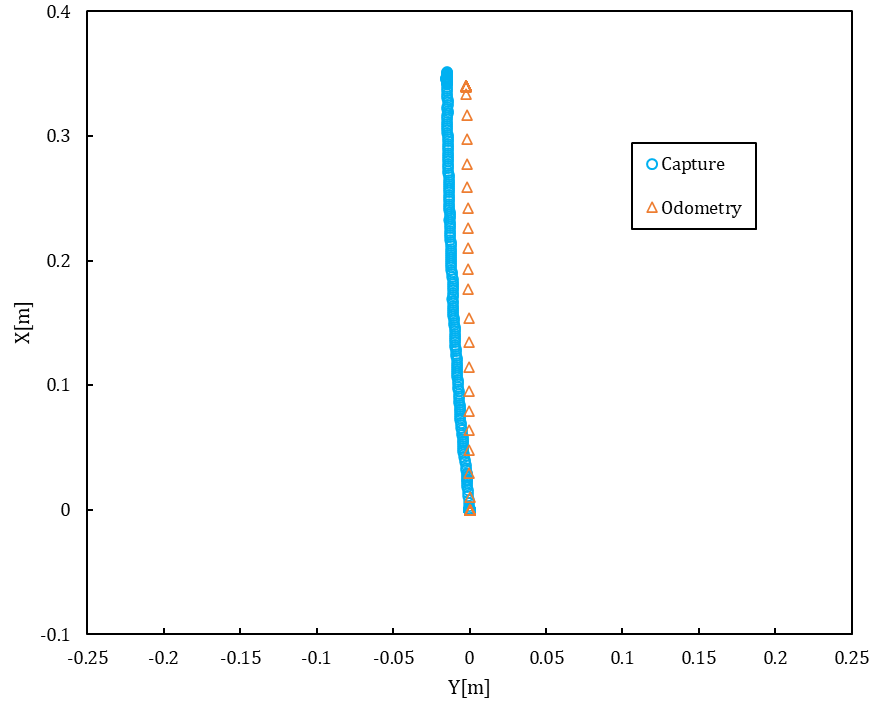
\includegraphics[width=100mm]{../graph/Xvs.Y.png}
        \caption{Roombaの軌跡}%図の説明
        \label{fig:1}
        \end{center}
\end{figure}
\begin{figure}[H] %\begin{figure}[画像の配置場所]
        \begin{center}
        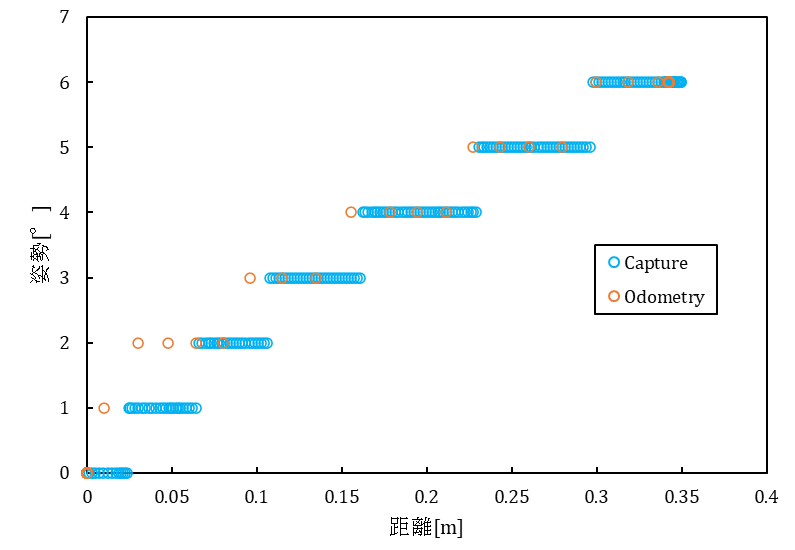
\includegraphics[width=100mm]{../graph/Rotationvs.Distance.png}
        \caption{距離と姿勢の関係}%図の説明
        \label{fig:2}
        \end{center}
\end{figure}
\begin{figure}[H] %\begin{figure}[画像の配置場所]
        \begin{center}
        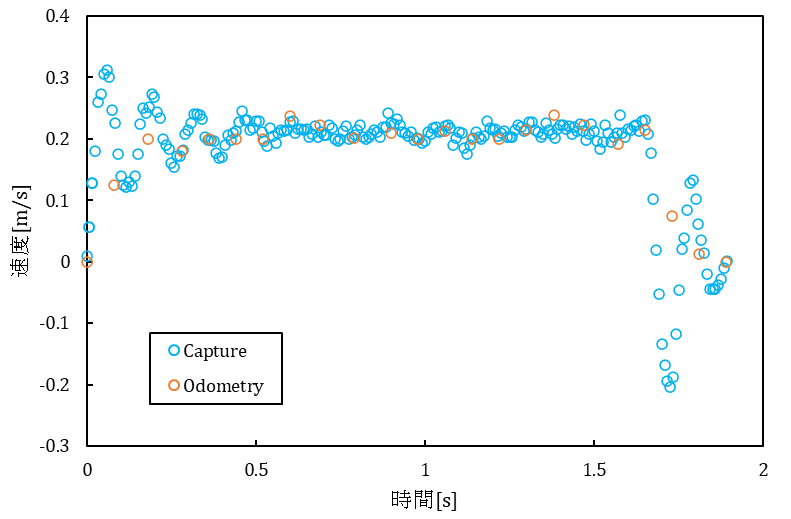
\includegraphics[width=100mm]{../graph/Velocityvs.Time.png}
        \caption{時間と速度の関係}%図の説明
        \label{fig:3}
        \end{center}
\end{figure}

\subsection{考察}
Fig.{\ref{fig:1}}より,オドメトリにより得られた軌跡とモーションキャプチャーにより得られた軌跡で差異が見受けられる.
この差異は,Fig.{\ref{fig:1}}の原点からX軸の正の方向に進むと大きくなっていることが分かる.
この差異は,Roombaのタイヤの滑りによって生じたものである.\par
Fig.{\ref{fig:2}}より,移動し始めた地点でのオドメトリによる姿勢は,モーションキャプチャーによる姿勢と比べ遅れて一致していることが分かる.
距離が大きくなるにつれ,姿勢が一致しやすくなっている.静止状態から走り始めは静止摩擦が大きく,その分大きなトルクが必要となる.
大きなトルクにより走り始めるため,タイヤが滑り姿勢もその分ずれが生じるためである.\par
Fig.{\ref{fig:3}}より,オドメトリによる速度は,定常的になるまでに徐々に速度が上昇しているが,
モーションキャプチャーでの速度は,定常的になるまで上昇と下降を繰り返しながら収束している.
また,Roombaが停止する地点1.89[s]より以前は,オドメトリでは徐々に速度が下降し0.00[m/s]を取るが,
モーションキャプチャーでは,速度が負の値と正の値を振動しながら0.00[m/s]に収束している.


\section{評価実験}
モーキャプと混ぜ合わせる,

\subsection{}

\section{}



\end{document}